\subsection{Nine directions}
\label{sec:nine-directions}
\label{sec:coherence}

The untied heading turns by $\turnMean^\circ$ at every boundary.
That alone does not say whether the nine blocks cooperate, ignore each other or work
against each other, and per-coordinate statistics cannot settle it, because the
feature basis is not privileged: rotating the channels changes them while leaving the
network's function intact (\cref{app:per-coordinate}).
We therefore use only quantities that depend on the Gram matrix of the block
increments, $G_{jk}=\langle\Delta x_j,\Delta x_k\rangle$ with
$\Delta x_k=x(k{+}1)-x(k)$, which is invariant to any orthogonal change of basis.
We compare three stages on the same $500$ validation images (one image from each of
$500$ classes drawn at random, seed $0$; massive channel removed): the weight-tied
and untied ConvNeXt-T, and a \emph{random} untied stage with Xavier weights whose gain
$g^\ast{=}1.35$ matches the per-block field strength $\|\Delta x_k\|/\|x_k\|$ of the
trained untied model.
\Cref{tab:coherence} collects the statistics and \cref{fig:transport} shows them per
block.

\begin{figure*}[t]
    \centering
    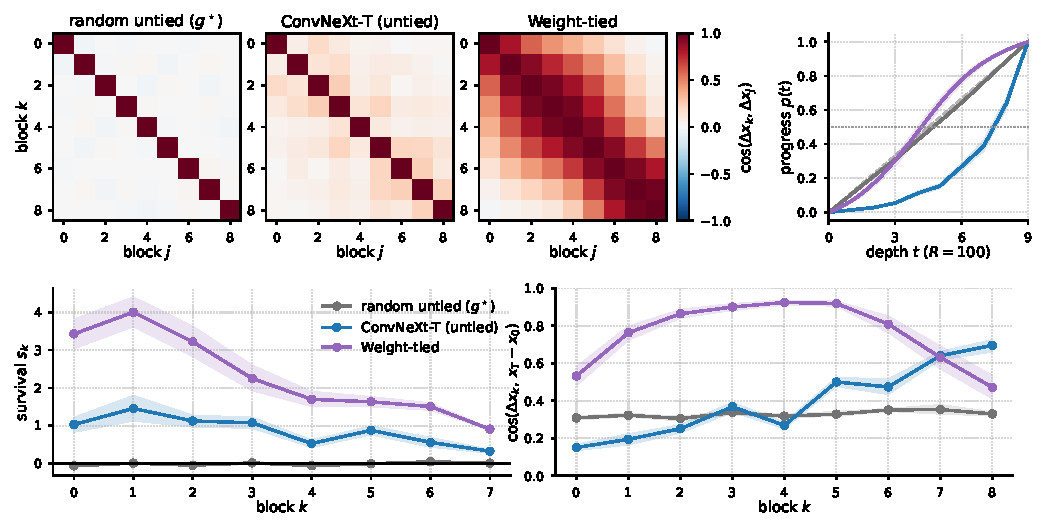
\includegraphics[width=\textwidth]{figures/transport_summary.pdf}
    \caption{Basis-independent transport statistics of stage~3 ($R{=}100$, $N{=}500$,
    massive channel removed).
    \textbf{Top left:} mean cosine between block increments $\Delta x_j$ and
    $\Delta x_k$ for a random untied stage of matched strength, the untied ConvNeXt-T
    and the weight-tied model.
    \textbf{Top right:} progress $p(t)$ along the chord $x_T-x_0$ (dashed: diagonal).
    \textbf{Bottom left:} survival $s_k$, the net projection of all later increments on
    $\Delta x_k$ in units of $\|\Delta x_k\|^2$ ($s_k<0$: later blocks oppose block $k$).
    \textbf{Bottom right:} alignment of each increment with the total displacement.
    Bands: P10--P90 over images.}
    \label{fig:transport}
\end{figure*}

\begin{table}[t]
    \centering
    \caption{Basis-independent transport statistics of stage~3, mean over $500$ images
    (std across images $\le 0.021$ for straightness and $\le 0.035$ for cosines).
    Str.: $\|x_T-x_0\|$ over path length (arc at $R{=}100$, chords at $R{=}1$);
    chords: $\|x_T-x_0\|$ over the sum of block chords;
    $\overline{\cos}$: mean off-diagonal cosine;
    $E$: opposed fraction; align: mean $\cos(\Delta x_k,x_T-x_0)$;
    $t_{50}$: first $t$ with $p(t)\ge 0.5$.}
    \label{tab:coherence}
    \scriptsize
    \setlength{\tabcolsep}{2.2pt}
    \resizebox{\linewidth}{!}{%
    \begin{tabular}{lrrrrrrrrr}
        \toprule
        & Str. & chords & $\cos_{k,k+1}$ & $\cos_{k,k+2}$ & $\overline{\cos}$ & $\min s_k$ & $E$ & align & $t_{50}$ \\
        \midrule
        Random $R{=}1$   & 0.330 & 0.330 & 0.001 & 0.002 & $-0.002$ & $-0.18$ & 0.022 & 0.330 & -- \\
        Random $R{=}100$ & 0.324 & 0.329 & $-0.001$ & $-0.001$ & $-0.004$ & $-0.19$ & 0.026 & 0.328 & \tFiftyRandom \\
        Untied $R{=}1$   & 0.501 & 0.501 & 0.165 & 0.136 & 0.093 & 0.11 & \EUntied & 0.393 & -- \\
        Untied $R{=}100$ & 0.502 & 0.510 & 0.171 & 0.143 & 0.099 & \sMinUntied & \EUntied & 0.394 & \tFiftyUntied \\
        Tied $R{=}1$     & 0.718 & 0.718 & 0.768 & 0.579 & 0.408 & 0.57 & \EUntied & 0.685 & -- \\
        Tied $R{=}100$   & 0.779 & 0.785 & 0.922 & 0.746 & 0.527 & 0.84 & \EUntied & 0.757 & \tFiftyTied \\
        \bottomrule
    \end{tabular}%
    }
\end{table}

\paragraph{Untied blocks write nearly orthogonal directions.}
Random residual blocks of matched strength write mutually orthogonal increments:
every off-diagonal cosine is $\cosRandom$ (\cref{fig:transport}, top left).
The trained untied blocks are not random: consecutive increments have cosine
$\cosUntied$ and increments two blocks apart $0.14$, all positive.
They are still far from the tied field, where consecutive increments have cosine
$\cosTied$ and remain correlated across the whole stage.
Each untied block therefore writes mostly in a new direction, slightly biased toward
the directions of its neighbours.

\paragraph{No block is erased.}
The survival $s_k=\sum_{j>k}G_{kj}/G_{kk}$ measures what later blocks do along the
direction of block $k$: $s_k>0$ means they continue it, $s_k<0$ that they move against
it and $s_k\le-1$ that they remove it entirely.
In the untied model $s_k$ is positive for every image and every block (minimum
$\sMinUntied$), so the opposed fraction $E$, the mass-weighted share of increments that
later blocks reverse, is exactly $\EUntied$.
Random blocks, by contrast, have $s_k<0$ in $61\%$ of the image and block pairs.
The untied stage is thus a staircase: each block adds a new, mostly orthogonal step
that no later block takes back.

\paragraph{A straightness ladder.}
Write $d=\|x_T-x_0\|$, $C=\sum_k\|\Delta x_k\|$ for the sum of block chords and $L$ for
the arc length of the refined path.
Straightness decomposes as
\begin{equation}
    \frac{d}{L} \;=\; \frac{d}{C}\,\frac{C}{L}.
    \label{eq:straightness-decomp}
\end{equation}
The factor $d/C$ is the between-block contribution (how aligned the chords are); $C/L$
is the within-block contribution (how much each block bends relative to its chord).
Straightness orders the three stages: $\strRandom$ for random blocks, $\strUntied$ for
untied blocks and $\strTiedNative$ to $\strTied$ for the tied field.
Nine orthogonal steps of equal length would give $1/\sqrt 9{=}0.33$, which is where the
random stage sits.
For the untied stage $C/L{=}\intraChordArcUntied$, so the arc is only
$\arcOverChordsPct\%$ longer than the sum of block chords; random blocks turn by a
similar amount ($0.987$) and the tied field by less ($0.993$).
The detour of the untied stage is made between blocks, not within them.

Per-coordinate sign changes between consecutive blocks ($\approx 45\%$) are what any
basis gives under a consecutive cosine of $\cosUntied$ (\cref{app:per-coordinate});
they are not evidence that some blocks reverse others.

\paragraph{Alignment with the destination.}
Projecting the path on the chord $x_T-x_0$ shows when progress is made
(\cref{fig:transport}, top right).
The untied stage crosses half of its net displacement at $t_{50}{=}\tFiftyUntied$, the
tied one at $\tFiftyTied$ and the random one at $\tFiftyRandom$, close to the linear
$4.5$.
Per block, the alignment $\cos(\Delta x_k,x_T-x_0)$ of the untied increments rises
from $\alignFirstUntied$ in the first block to $\alignLastUntied$ in the last, while
the random stage stays at $0.33$ and the tied field peaks at $0.92$ mid-stage
(\cref{fig:transport}, bottom right).
Early untied blocks write directions that are almost orthogonal to where the stage
ends; the last blocks write most of the final displacement.

\paragraph{Other architectures.}
The staircase is not universal (\cref{app:arch-transport}).
Swin-T stage~3 is coherent, with straightness $0.80$ ($0.67$ without the corner
tokens) against $0.42$ for random blocks and positive survival everywhere.
ResNet-50 and ResNet-101, whose stage-3 residual includes the ReLU after the sum, go the
other way: straightness $0.37$ and $0.16$, below their random baselines of $0.43$ and
$0.22$ to $0.23$, with genuine reversal ($E$ of $0.19$ and $0.24$ against about
$0.07$--$0.09$ for their random baselines).
We have not tested whether the post-sum ReLU explains that reversal.
